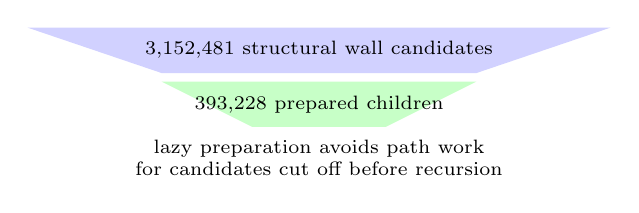
\begin{tikzpicture}[x=1cm,y=0.72cm,font=\scriptsize]
\fill[blue!18] (0,2) -- (7.4,2) -- (5.7,1.2) -- (1.7,1.2) -- cycle;
\fill[green!22] (1.7,1.05) -- (5.7,1.05) -- (4.55,0.25) -- (2.85,0.25) -- cycle;
\node at (3.7,1.62) {3,152,481 structural wall candidates};
\node at (3.7,0.65) {393,228 prepared children};
\node[align=center] at (3.7,-0.3) {lazy preparation avoids path work\\for candidates cut off before recursion};
\end{tikzpicture}
